%%%%%%%%%%%%%%%%%%%%%%%%%%%%%%%%%%%
%\documentclass[prd,aps,twocolumn,nofootinbib,showpacs,superscriptaddress]{revtex4-1}
\documentclass[prd,twocolumn,nofootinbib]{revtex4-1}
%\documentclass[prd,aps,nofootinbib,showpacs]{revtex4-1}
\usepackage{amsfonts}
\usepackage{amsmath}
\usepackage{amssymb}
\usepackage{bm}
\usepackage{dcolumn}
\usepackage[dvips]{graphicx}
\usepackage{graphics}
%\usepackage[latin1]{inputenc}
\usepackage{latexsym}
\usepackage{rotating}
\usepackage[colorlinks=true]{hyperref}
\usepackage{xspace} % Sensible space treatment at end of simple macros
\usepackage[usenames]{color}
\usepackage{mathrsfs}
\usepackage{multirow}
\usepackage{pifont}
\usepackage{enumitem}
\usepackage{color}
\usepackage{ulem}
\usepackage{url}
\usepackage{appendix}
\usepackage[utf8]{inputenc}
%\usepackage[toc,page]{appendix}
\usepackage{comment}
%% Try to control orphans, widows, and extra whitespace
\widowpenalty=1000
\clubpenalty=1000
\raggedbottom

\definecolor {darkgreen}{rgb}{0.2,0.7,0.2}
\definecolor{purple}{rgb}{0.5,0,0.5}

\newcommand\be{\begin{equation}}
\newcommand\ba{\begin{eqnarray}}
\newcommand\ee{\end{equation}}
\newcommand\ea{\end{eqnarray}}
\newcommand\bw{\begin{widetext}}
\newcommand\ew{\end{widetext}}
\newcommand{\lb}{\left(}
\newcommand{\rb}{\right)}

\newcommand{\EDGB}{{\mbox{\tiny EdGB}}}
\newcommand{\BD}{{\mbox{\tiny BD}}}
\newcommand{\NC}{{\mbox{\tiny NC}}}
\newcommand{\PPE}{{\mbox{\tiny ppE}}}
\newcommand{\KG}{{\mbox{\tiny kh}}}
\newcommand{\EA}{{\mbox{\tiny EA}}}
\newcommand{\ST}{{\mbox{\tiny ST}}}
\newcommand{\NS}{{\mbox{\tiny NS}}}
\newcommand{\DCS}{{\mbox{\tiny dCS}}}
\newcommand{\GR}{{\mbox{\tiny GR}}}
\newcommand{\Gdot}{{\mbox{\tiny $\dot G$}}}
\newcommand{\GW}{{\mbox{\tiny GW}}}
\newcommand{\ky}[1]{\textcolor{blue}{\it{\textbf{ky: #1}}} }
\newcommand{\kent}[1]{\textcolor{magenta}{\textbf{#1}} }
\newcommand{\st}[1]{\textcolor{cyan}{\it{\textbf{st: #1}}} }

%\bibliographystyle{apsrev}
\begin{document}
\title{Not decided yet}

\author{Sharaban Tahura}
\affiliation{Department of Physics, University of Virginia, Charlottesville, Virginia 22904, USA.}

\author{Kent Yagi}
\affiliation{Department of Physics, University of Virginia, Charlottesville, Virginia 22904, USA.}

\author{Zack Carson}
\affiliation{Department of Physics, University of Virginia, Charlottesville, Virginia 22904, USA.}

\begin{abstract}
\ky{I added Zack in the author list. Somewhere in the paper, we need to show the comparison of the PPE bounds with PhenomB (that you computed) and PhenomD (that Zack computed) to justify the use of PhenomB for negative PN corrections.}

To be written later
\end{abstract}

\date{\today}




\maketitle


%%%%%%%%%%%%%%%%%%%%%%%%%%


\section{Introduction}

\section{PPE Formalism}\label{section:ppE}

\section{Data Analysis Formalism}
%Fisher Analysis
%%Assumptions
We adopt a Fisher analysis~\cite{Cutler:1994ys} to estimate the statistical errors of the non-GR parameters in various theories. Such an analysis is valid for GW events with sufficiently large signal-to-noise (SNR) ratios. We make the assumptions that the detector noise is Gaussian and stationary. Let us write the detector output as
\be
s(t)=n(t)+h(t)\,,
\ee
where $n(t)$ and $h(t)$ are the noise and the GW signal respectively. Let us also define the inner product of two quantities $A(t)$ and $B(t)$ as
 \be
 \left(A|B\right)=4\Re\int_0^\infty df \frac{\tilde{A}^*(f)\tilde{B}(f)}{S_n \left( f \right)}\,.
 \ee
Here $\tilde{A}(f)$ is the Fourier component of $A$, an asterisk ($*$) superscript means the complex conjugate and $S_n\left(f\right)$ is the noise spectral density. With the above definitions, the probability distribution of the noise can be written as
 \be
P\left(n=n_0(t)\right) \propto \text{exp}\left[-\left(n_0|n_0\right)\right]\,,
\ee
and the SNR for a given signal $h(t)$ can be defined as
\be
\rho \equiv\sqrt{\left(h|h\right)}\,.
\ee
Under the assumptions of a Gaussian and stationary noise, the posterior probability distribution of binary parameters $\theta^a$ takes the following form:
\be
P\left(\theta^a|s\right) \propto p^{(0)}\left(\theta^a\right) \text{exp}\left[-\frac{1}{2} \Gamma_{ab} \Delta\theta^a\Delta \theta^b \right]\,,
\ee
where $\Delta \theta^a=\hat{\theta}^a-\theta^a$ with $\hat{\theta}^a$ being the maximum likelihood values of $\theta^a$. $p^{(0)}\left(\theta^a\right)$ gives the probability distribution of the prior information, \kent{which we take to be in a Gaussian form for simplicity}. $\Gamma_{ab}$ is called the Fisher information matrix which is defined as
\be
\Gamma_{ab}=\left(\partial_a h|\partial_b h \right)\,,
\ee
where $\partial_b\equiv \frac{\partial}{\partial \theta^b}$. One can estimate the root-mean-square of $\Delta \theta^a$ by taking the square root of the diagonal elements of the inverse Fisher matrix $\Sigma^{ab}$: 
\be
\Sigma^{ab}=\left(\tilde{\Gamma}^{-1}\right)^{ab}=\langle\Delta\theta^a\Delta \theta^b\rangle\,,
\ee
where $\tilde{\Gamma}_{ab}$ is defined by
\be
p^{(0)}\left(\theta^a\right) \text{exp}\left[-\frac{1}{2} \Gamma_{ab} \Delta\theta^a\Delta \theta^b \right]=\text{exp}\left[-\frac{1}{2} \tilde{\Gamma}_{ab} \Delta\theta^a\Delta \theta^b \right]\,.
\ee

%%binary parameters
We choose the following parameters as our variables for the Fisher analysis:
\bw
\ba
\theta^a\equiv \lb \ln{\mathcal{M}_z}, \ln{\eta}, \ln{D_L}, \ln{t_0}, \chi, \phi_0, \alpha, \delta, \psi, \theta_{\text{inc}}, \beta_{\PPE}, \alpha_{\PPE} \rb\,.
\ea
\ew
Here, $\mathcal{M}_z$ is the the redshifted chirp mass and $\chi$ is the effective spin parameter~\footnote{The effective spin parameter is defined as $\chi\equiv\lb m_1 \chi_1+m_2\chi_2\rb /\lb m_1+m_2\rb$, where $\chi_A$ with $A=(1,2)$ is the dimensionless spin of the $A$th body.}. $\alpha, \delta, \psi$, and  $\theta_{\text{inc}}$ are the right ascension, declination, polarization and inclination angles respectively in the detector frame. All other parameters have the same meanings as in Sec.~\ref{section:ppE}. 
%Monte-Carlo
We perform a Monte Carlo simulation by using each set of the posterior samples released by LIGO~\cite{ligo:sample} for $(\mathcal{M}_z, \eta, D_L, \chi, \alpha, \delta$, $\theta_{\text{inc}})$, while we randomly sample the polarization angle $\psi$ and the coalescence phase $\phi_0$ in $[0,\pi]$ and $[0,2\pi]$ respectively.
%%prior on spin
We impose the prior information such that the effective spin is less than 1.

%%Detectors
We use the detector sensitivity of Advanced LIGO (aLIGO) O1 run~\cite{LIGOScientific:2018mvr} and we consider the two detectors at Hanford and Livingstone. For simplicity, we assume that the Livingstone noise spectrum is identical to that of the Hanford~\cite{Yunes:2009yz}. For Fisher integration, the minimum frequency is taken to be 20 Hz while the maximum frequency is same as the cutoff frequency above which the signal power is negligible~\cite{Ajith:2009bn}.


%The rule of compound probability
Now we are going to discuss how we achieve the probability distribution of a non-GR parameter from the output of a Fisher analysis with a Monte Carlo simulation. We set the  fiducial value of any non-GR parameter to be zero for our analysis. We perform the following integration numerically to obtain the compound probability density function~\footnote{If the distribution of a random variable $y$ depends on a parameter $x$, and if $x$ is not fixed rather a random variable, the marginal distribution of $y$ is called mixture distribution or compound probability distribution and is given by $P\left(y\right)=\int P\left(y|x\right) P\left(x\right)dx$. The underlying distribution $P\left(x\right)$ is called mixing distribution or latent distribution.~\cite{2016arXiv160204060R}} of any parameter $\xi$~:
\be
\label{eq3:1}
P\lb\xi\rb=\int P\lb \xi|\sigma_{\xi}\rb P\lb \sigma_{\xi}\rb d\sigma_{\xi}\,,
\ee
where $P\lb\xi\rb$ is the marginal (unconditional) probability density function of $\xi$. $P\lb \xi|\sigma_{\xi}\rb \propto \exp[-(\xi-\bar \xi)^2/2\sigma_{\xi}^2]$ is the conditional probability density function of $\xi$ which we assume to be a Gaussian distribution with a mean $\bar \xi$ and a standard deviation $\sigma_\xi$. $P\lb\sigma_\xi\rb$ is the probability distribution of $\sigma_\xi$ computed from the Fisher analysis for the entire posterior distribution.
%We perform the integration in Eq.~\ref{eq3:1} numerically to obtain the unconditional probability density function $P\lb\xi\rb$.
\section{Example Theories}
\subsection{Einstein-Dilaton-Gauss-Bonnet Gravity}
%Introduction
%%Importance
EdGB gravity endows one of the simplest high-energy modification to GR~\cite{Moura:2006pz,Pani:2009wy}. Such a theory is motivated from low-energy effective string theories and also arises as a special case of Horndeski gravity~\cite{Zhang:2017unx,Berti:2015itd}. 
%%Definition
\sout{One obtains} The EdGB action \kent{is given by introducing} \sout{by adding} a quadratic-curvature correction \kent{(Gauss-Bonnet invariant)} to the GR action \sout{while the correction is achieved by} \kent{that is} non-minimally \kent{coupled to} a scalar field (dilaton) \sout{to the Gauss-Bonnet term} with a coupling constant $\bar{\alpha}_\EDGB$~\cite{Kanti:1995vq}\footnote{We use barred quantities for coupling constants in order to distinguish them from the PPE parameters.}.
%%Existing bounds

%ppE parameters
In EdGB gravity, BHs acquire scalar monopole charges which may generate scalar dipole radiation \kent{if they form binaries}~\cite{Yagi:2011xp,Sotiriou:2014pfa,Berti:2018cxi,Prabhu:2018aun}. Such radiation leads to an earlier coalescence of BH binaries compared to that of GR and modifies the \sout{GW phase} \kent{gravitational waveform} with the PPE parameters given by~\cite{Yunes:2016jcc,Yagi:2011xp}
\begin{equation}
 \beta_\EDGB=-\frac{5}{7168}\zeta_\EDGB\frac{(m_1^2\tilde s_2^\EDGB-m_2^2\tilde s_1^\EDGB)^2}{m^4\eta^{18/5}}\,,
 \end{equation}
 with $b=-7$ and 
  \begin{equation}
 \alpha_\EDGB=-\frac{5}{192}\zeta_\EDGB\frac{(m_1^2 \tilde s_2^\EDGB-m_2^2 \tilde s_1^\EDGB)^2}{m^4\eta^{18/5}}\,,
 \end{equation}
 with $a=-2$.  Here, $\zeta_\EDGB\equiv 16 \pi \bar{\alpha}_\EDGB^2/m^4$ is the dimensionless EdGB coupling parameter and $\tilde s_{A}^\EDGB$ are the spin-dependent factors of the BH scalar charges given by $\tilde s_{A}^\EDGB\equiv 2(\sqrt{1-{\chi_A}^2}-1+{\chi_A}^2)/{\chi_A}^2~$~\cite{Berti:2018cxi,Prabhu:2018aun}\footnote{For ordinary stars like NSs $\tilde s_A^\EDGB$ are zero~\cite{Yagi:2011xp,Yagi:2015oca}.}.

\begin{figure}[htb]
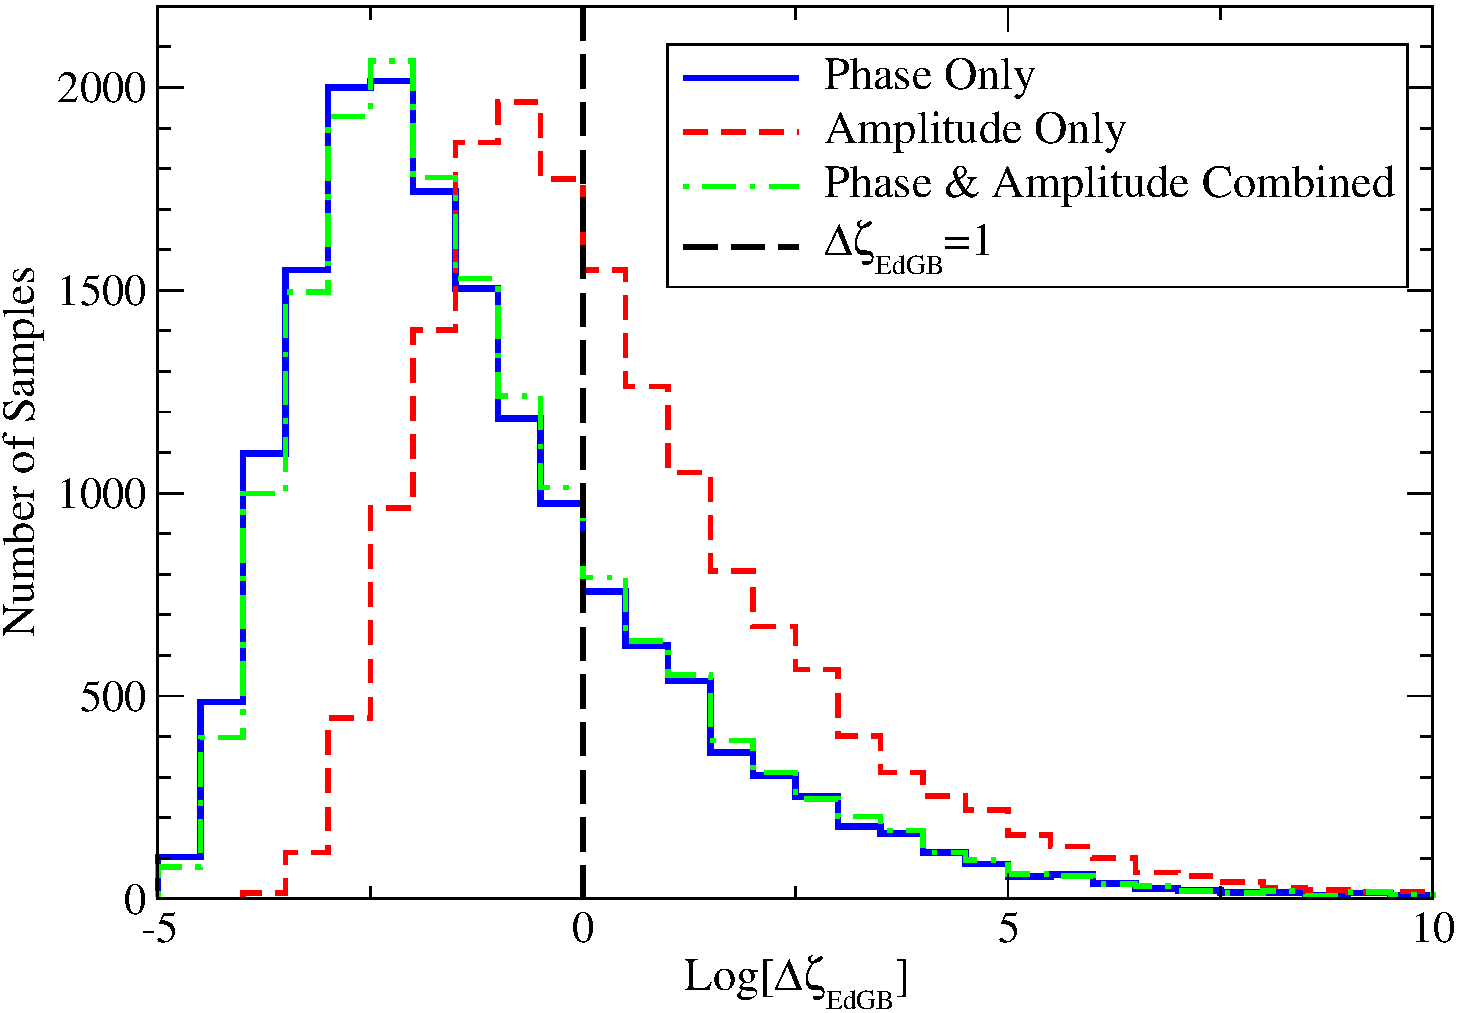
\includegraphics[width=8.5cm]{histogram-gw150914.eps}
\caption{Histogram distributions of \kent{the 90\% CL bounds on} $\zeta_{\EDGB}$ from \kent{a Fisher analysis with the phase correction only (blue solid), the amplitude correction only (red dashed) and combining the two corrections (green dotted-dashed). Fiducial values are taken from} the posterior \sout{distribution} \kent{samples} of GW150914. \sout{The horizontal axis shows the Logarithm of $\Delta\zeta_{\EDGB}$,  where $\Delta\zeta_{\EDGB}$ is the 90\% CL constraint obtained from a Fisher analysis. The vertical axis shows the number of samples that produce a particular value of $\Delta\zeta_{\EDGB}$.} The samples that lie on the left side of the vertical black dashed line satisfy \kent{the} small coupling approximation with 90\% CL.}
\label{fig:histogram-edgb}
\end{figure}


%Small coupling approximation
We now derive constraints on EdGB gravity from GW150914 and GW151226. First we \sout{want to} estimate how well those events satisfy the small coupling approximation $\zeta_{\EDGB}<1$. \sout{In order to do that} \kent{To do so,} we extract the 90\% CL upper bound $\Delta\zeta_{\EDGB}$ from each sample of the posterior distribution of a particular event. \sout{Then} We \kent{then create} \sout{make a} histograms \sout{plot} with all the samples (see Fig.~\ref{fig:histogram-edgb}) and calculate the fraction \sout{of the samples} satisfying $\Delta\zeta_{\EDGB}<1$.  For GW150914, 72\% \kent{(40\%)} of the samples satisfy \kent{the} small coupling approximation if $\Delta\zeta_{\EDGB}$ is derived from \kent{the} phase \kent{(amplitude)} correction, while \sout{for amplitude correction it is only 42\%. On the other hand,} 70\% of the posterior distribution satisfies such approximation if \kent{the} phase and amplitude corrections are combined. A similar analysis with GW151226 gives 98\% and 87\% for the phase and amplitude corrections respectively while combining \sout{phase with amplitude produces} \kent{the two yields almost} the same result as that of the phase-only case. Since the fraction of samples satisfying $\zeta_{\EDGB}<1$ is much higher for GW151226 than GW150914 \kent{due to a larger number of GW cycles and slower relative velocity of binary constituents}, the former event places more reliable constraints on EdGB gravity compared to the latter one.


\begin{figure}[htb]
\includegraphics[width=8.5cm]{edgb-gw150914.eps}
\caption{\ky{Please add a bar on top of $\alpha$ on the horizontal axis label.}
Cumulative probability distributions of $\bar{\alpha}^2_{\EDGB}$ obtained from GW150914 for \sout{three different cases: phase-only, amplitude-only, and phase and amplitude combined. } \kent{the same three cases as in Fig.~\ref{fig:histogram-edgb}.} \sout{The horizontal axis gives the upper bound on $\bar{\alpha}^2_{\EDGB}$ while the vertical axis gives the corresponding cumulative probability.} \ky{I'm removing this sentence since it's just a repetition of the first line.} \kent{Each} vertical dashed line shows the \kent{corresponding} 90\% CL upper bound of a solid line of the same color.}
\label{fig:pdf-edgb}
\end{figure}


%Results
\kent{Figure~\ref{fig:pdf-edgb} presents cumulative probability distributions of $\bar{\alpha}^2_{\EDGB}$\footnote{\kent{We show the distribution of $\bar{\alpha}^2_{\EDGB}$ instead of $\sqrt{\bar{\alpha}_{\EDGB}}$ as it is the former that directly enters in the waveform.}} for GW150914 for three different cases with vertical lines showing the 90\% CL of the corresponding distribution. We found}
\sout{Following the formula in Eq.~\eqref{eq3:1} we compute the probability distribution of $\bar{\alpha}^2_{\EDGB}$ for GW150914 (see Fig.~\ref{fig:pdf-edgb}) and extract} the 90\% CL constraints on  $\sqrt{\bar{\alpha}_{\EDGB}}$ from \kent{each of} the phase and amplitude corrections as 50.5 km and 76.3 km respectively. Notice that these bounds \sout{from phase and amplitude} have the same order of magnitude. On the other hand, combining the amplitude and phase corrections leads to an upper bound of 51.5 km, which is \sout{larger} \kent{weaker} than the  phase-only constraint by 2\%.
Similar analyses with GW151226 yield 4.3 km and 10.5 km respectively from \kent{the} phase and amplitude \kent{corrections},
%\footnote{The upper bound on $\sqrt{\bar{\alpha}_{\EDGB}}$ derived from the phase correction with GW151226 agrees with those of ref.~\cite{Nair:2019iur} and~\cite{Yamada:2019zrb}}, 
while \kent{combining the two only changes the result from including only the phase correction by 0.01\%.} \sout{the difference between the phase-only case and the combined analysis  is only 0.01\%. As we can see,} 
\kent{These bounds are consistent with those in a recent paper~\cite{Nair:2019iur} while Ref.~\cite{Yamada:2019zrb} found even stronger bounds by combining multiple GW events. These GW bounds are comparable to the one obtained from low-mass X-ray binaries~\cite{Yagi:2012gp}.}
Although GW150914 leads to \sout{worse} \kent{weaker} \ky{Try to avoid using ``good'' and ``bad'' but use more specific adjectives instead.} constraints on EdGB gravity compared to GW151226, the effect of amplitude correction is more manifest for the former event. \kent{This is because GW150914 has a smaller number of GW cycles and thus the amplitude contribution becomes relatively higher than GW151226.}

\ky{I added this paragraph.}
Why does the inclusion of the amplitude correction deteriorates the bound slightly from the case where one only includes the phase correction? This may sound counter-intuitive as one might think adding more EdGB corrections should improve the bound. Indeed, if one neglects correlations among $\bar \alpha^2_\EDGB$ and other binary parameters, addition of the amplitude correction improves the bound. However, such amplitude correction introduces a strong correlation between $\bar \alpha^2_\EDGB$ and the luminosity distance. As a result, the bound derived by including both the amplitude and phase corrections becomes weaker than that from the latter only.


\subsection{Massive Gravity}
\subsection{Varying- $G$ Theory}
\subsection{Scalar-Tensor Theories}
\section{Conclusion}
\section{Appendix}
%phenomB vs PhenomD for generation mechanism
%------------------------------------------------------- 
\bibliography{ppE}
\end{document}
